\documentclass{standalone}
\usepackage{tikz}
%x step={
\usetikzlibrary{positioning}
%x }
\usetikzlibrary{decorations.pathreplacing}

\begin{document}

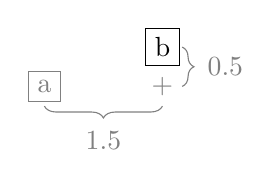
\begin{tikzpicture}
%x description="nodes with relative positioning (4)"
%x pre={
\node[draw, gray] (a) at (0,0) {a};
%x }

%x step={
\node[draw] (b) [on grid, above right=0.5 and 1.5 of a] {b};
%x }

\tikzset{brace/.style={decorate, decoration={brace, amplitude=0.15cm}, gray}}
\draw[brace]
	(b.center |- a.center) ++ (0,-0.25)
	-- node [below=0.2] {1.5}
	+(-1.5,0);

\draw[brace]
	(b.center |- a.center) ++ (0.25,0.5)
	-- node [right=0.2] {0.5}
	+(0,-0.5);

\node[gray] at (a.center -| b.center) {+};

\end{tikzpicture}

\end{document}
